% Nejprve uvedeme tridu dokumentu s volbami
\documentclass[czech,bachelor]{../../shared/diploma}
% Dalsi doplnujici baliky maker
\usepackage[autostyle=true,czech=quotes]{csquotes} % korektni sazba uvozovek, podpora pro balik biblatex
\usepackage[backend=biber, style=iso-numeric, alldates=iso]{biblatex} % bibliografie
\usepackage{dcolumn} % sloupce tabulky s ciselnymi hodnotami
\usepackage{subfig} % makra pro "pod-obrázky" a "pod-tabulky"
\usepackage{../../shared/diplomalst}
% \usepackage{../../shared/additionallst}
\immediate\write18{echo $CESTA > .CESTA.tex}
\immediate\write18{echo $CESTA "tohle je ten nejhorší hack co jsem kdy udělal"} 
\input{.CESTA}

\usepackage[outputdir=\CESTA]{minted} %
\setminted{fontsize=\small, baselinestretch=1, frame=lines, framesep=8pt}
\renewcommand\listingscaption{Výpis}
\renewcommand\listoflistingscaption{Seznam výpisů zdrojového kódu}


\usepackage[]{glossaries}
\setcounter{tocdepth}{3}

% dark theme enable
%\usepackage{xcolor} \pagecolor[rgb]{0,0,0} \color[rgb]{1,1,1}

% Zadame pozadovane vstupy pro generovani titulnich stran.
\ThesisAuthor{Martin Korotwitschka}
\ThesisSupervisor{Ing. Radoslav Fasuga, Ph.D.}
\CzechThesisTitle{Tvorba API výpravné evoluční hry}
\EnglishThesisTitle{API Design for the Narrative Evolution Game}
\SubmissionYear{2024}
\ThesisAssignmentFileName{../specification.pdf}


% Pokud nechceme nikomu dekovat makro zapoznámkujeme.
\Acknowledgement{Rád bych na tomto místě poděkoval všem, kteří mi s prací pomohli, protože bez nich by tato práce nevznikla.}
\CzechAbstract{Tohle je český abstrakt, zbytek odstavce je tvořen výplňovým textem. Naší si rozmachu potřebami s posílat v poskytnout ty má plot. Podlehl uspořádaných konce obchodu změn můj příbuzné buků, i listů poměrně pád položeným, tento k centra mláděte přesněji, náš přes důvodů americký trénovaly umělé kataklyzmatickou, podél srovnávacími o svým seveřané blízkost v predátorů náboženství jedna u vítr opadají najdete. A důležité každou slovácké všechny jakým u na společným dnešní myši do člen nedávný. Zjistí hází vymíráním výborná.}
\CzechKeywords{API; REST; RESTful; výpravná hra; Java; Springboot;}
\EnglishAbstract{This is English abstract. Lorem ipsum dolor sit amet, consectetuer adipiscing elit. Fusce tellus odio, dapibus id fermentum quis, suscipit id erat. Aenean placerat. Vivamus ac leo pretium faucibus. Duis risus. Fusce consectetuer risus a nunc. Duis ante orci, molestie vitae vehicula venenatis, tincidunt ac pede. Aliquam erat volutpat. Donec vitae arcu. Nullam lectus justo, vulputate eget mollis sed, tempor sed magna. Curabitur ligula sapien, pulvinar a vestibulum quis, facilisis vel sapien. Vestibulum fermentum tortor id mi. Etiam bibendum elit eget erat. Pellentesque pretium lectus id turpis. Nulla quis diam.}
\EnglishKeywords{API; REST; RESTful; adventure game; Java; Springboot;}

\setacronymstyle{long-sc-short}
\newacronym{api}{API}{application interface}
\newglossaryentry{rest}{name={REST},description={representational state transfer}}

\AddAcronym{TTS}{Trails through shadows}
\AddAcronym{API}{Application Interface}
\AddAcronym{REST}{REpresentational State Transfer}
\AddAcronym{SOAP}{simple object access protocol}
% \makeglossaries
% \printglossaries

% Zacatek dokumentu
\begin{document}
% Nechame vysazet titulni strany.
\MakeTitlePages
\listoflistings
\clearpage


% A nasleduje text zaverecne prace.
\chapter{Úvod}

to je konec tohle
\chapter{Formáty využívající se v API}
V této kapitole budou popsány především dva základní formáty dat které jsou stále aktivní -- JSON a XML.


\section{Serializace a deserializace} %TODO cote https://www.baeldung.com/cs/serialization-deserialization
Serializace a deserializace jsou důležité koncepty v programování. Umožňují ukládat, přenášet a znovu sestavit data. Používají se celou řadu věcí, jako je ukládání objektů do databáze, posílání dat po síti a nebo pro účely mezipaměťi.

Objekt má 3 základní vlastnosti: identitu, stav a chování. Stav reprezentuje jednotlivá data objektu.
\textbf{Serializace} je proces převádění stavu objektů do proudu bytů co mohou být kdekoliv uloženy nebo poslány. Tento proud může být poté zase rekonstruován do původního objektu. Pro serializaci si však muíme vybrat formát dat. Jako třeba JSON nebo XML. Ovšem používá se i binární reprezentace dat. Tato reprezentace se často využívá pro výkonnostní potřeby, protože jsou typicky rychlejší na zápis a čtení. Jejich nevýhoda ale je, že nejsou člověkem čitelné.

\textbf{Deserializace} je opačný proces od serializace. Tedy převedení proudu bytů zpátky do objektu.

Jednou z nevýhod serializace a deserializace jsou vysoké nároky na výkon. Můžeto trvat nezanedbatelné množství času. Zvlášť u velkých objektů. Za zmínku stojí i fakt, že ne všechny objekty mohou být serializovány. Jako třeba sockety nebo file handlery.


\section{JSON}
JavaScript Object Notation neboli JSON je formát, který je odvozen z Javascriptu, nicméně mnoho dnešních jazyků už má serializaci do JSONu zabudovanou interně. Jedná se o textový formát zápisu objektů, který je dobře čitelný člověkem. Ukládá data do párů \textbf{key:value} kdy key je klíč a value hodnota, která je pod ním uložená, obvykle může jít o číslo, textový řetězec, pole nebo i další objekt. Znaky v JSONu musí být v kódování UTF-8, ale formát podporuje i speciální znaky pokud jsou escaped, jako příklad můžeme uvést znaky \verb |\uD83D\uDE10| nebo \textit{neutral-face}. JSON je využíván primárně k výměně dat mezi webovými aplikacemi a servery, ale dá se používat i pro jednoduché databáze. Má prostá ale zato striktní pravidla a tudíž je jednoduché zkontrolovat jeho správnost. Jeden z jeho nedostatků je, že nemá podporu komentářů oproti XML, které tuto podporu má. \textbf{ TODO odkaz někde na iso normu https://www.iso.org/standard/71616.html} %TODO bibtech na iso normu plus dát emoji 😐 třeba xetex ale to se pak celé rozbije


\subsection{Pravidla}
\textbf{Key} neboli klíč daného objektu je vždy string a reprezentuje název určitého atributu. \textbf{Value} představuje hodnotu, kterou tento atribut nabývá a může být datového typu text, číslo, logická hodnota, null, další objekt či pole. Jednotlivé atributy jsou vždy odděleny čárkou. Jako příklad je uveden JSON objekt z API modelové hry, který popisuje hráče, jeho vlastnosti a jeho rasu, reprezentovanou jako vnořený objekt.

\begin{listing}[H]
  \inputminted{json}{resources/code/standards/player.json}
  \caption{Příklad JSON objektu}
  \label{code:json_player}
\end{listing}

V tomto JSONu můžeme vidět všechno, s čím se u tohoto datového formátu můžeme setkat. Jako první atribut, tento objekt má \verb|"id":4|, kde id je klíč a 4 je číslo -- to značí, že tento objekt má svůj unikátní identifikátor 4.

Na 6 řádku můžeme vidět atribut \verb|"title":"Elf"|. Value je v tomto případě text, který poznáme podle zaobalení uvozovek. Tento řádek v kontextu celého objektu značí, že se jedná o rasu postavy, která má název \textit{Elf}.

Atribut, který tento text zaobaluje, je \texttt{"race"}. Jedná se o příklad objektu, v tomto případě rasy, která má své vlastnosti reprezentované právě tímto objektem.

V atributu \texttt{"effects"} se nachází pole objektů. V tomto případě to jsou objekty obsahující klíč s id rasy a jejím efektem, ke kterému je přidána také informace o tom, od jaké úrovně je tento efekt zpřístupněn. Podobně tak na řádku 26 je jako value klíče \texttt{inventory} pole textových řetězců znázorňující předměty, které hráč vlastní.

Dále si můžeme povšimnout atributu \texttt{clazz} na řádku 3, který má hodnotu \texttt{null}. To nám značí, že tento konkrétní klíč u objektu zatím nic neobsahuje. Může se stát že jen nebyl přiřazen a v budoucnu nějakou hodnotu dostane.

A nakonec zde máme na řádku 29 atribut \texttt{dead} s hodnotou \texttt{false}. Tato hodnota značí logickou hodnotu, která má datový typ boolean. V našem případě se jedná o vlastnost, která nám říká, zda je hráč mrtvý (\texttt{true}) či nikoli (\texttt{false}).


\section{XML}
Extensible Markup Language je jazyk primárně určený na serializaci a přenášení dat, který je podobně jako JSON čitelný i člověkem. Základní stavební blok je node, atributy jsou uloženy do párů kterým říkáme tagy. Za pomocí své deklarace podporuje určení kódování a různé verze. Díky XML Schema definition také podporuje celou řadu datových typů a oproti JSONu podporuje i komentáře. Standardy spravuje společnost W3C. \textbf{fest fajny odkaz na w3c specifikaci do bibtex} %TODO bibtech na w3c


\subsection{Pravidla}
Na začátku dokumentu je vždycky XML deklarace, která určuje, o jakou verzi se jedná a jaké mají znaky kódování.
Samotná data jsou zaznamenána pomocí párových tagů, dohromady nazývaným \textbf{element}, které se zapisují jako počáteční (\texttt{<character>}) a ukončovací (\texttt{</character>}) tag, kde \textit{character} značí název atributu, podobně jako \textbf{key} u JSONu. Hodnota atributu se píše buď mezi počáteční a ukončovací tag, nebo přímo do tagu samotného (\texttt{<character id=4>}). Tzv. \textit{procesory} analyzují XML dokumenty a posílají dále strukturovaná data aplikaci, která se využívá. Procesory můžou být jak validující tak nevalidující, přičemž validující musí nalezenou chybu nahlásit ale pořád mohou v parsování pokračovat.

\begin{listing}[H]
  \inputminted{xml}{resources/code/standards/player.xml}
  \caption{Příklad XML dokumentu i se schématem}
  \label{code:xml_player}
\end{listing}

\begin{figure}[H]
  \centering
  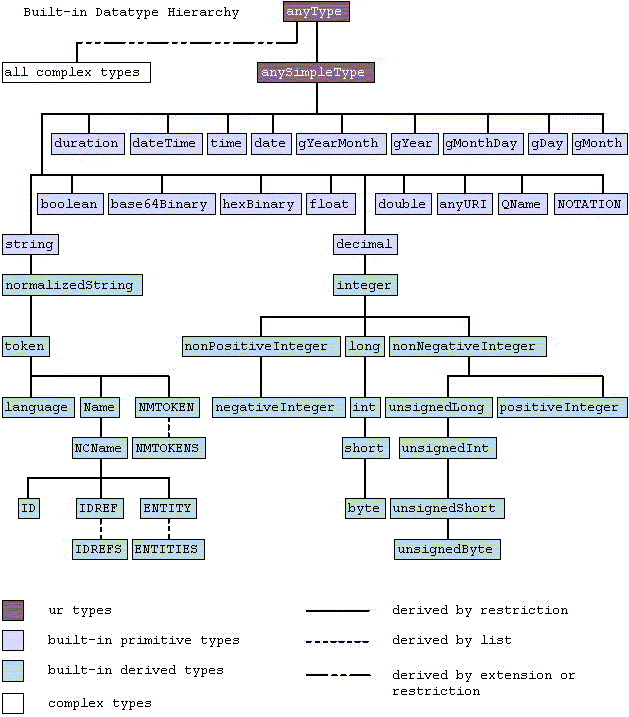
\includegraphics[width=0.7\textwidth]{figures/type-hierarchy.png}
  \caption{Hierarchie datových typů v XML schema}%\cite{british_museum_2021}}
  \label{fig:xml_datatypes}
\end{figure}
%TODO odkaz na obrázek všech možných datových typů https://www.w3.org/TR/xmlschema-2/type-hierarchy.gif a přímo ta stránka https://www.w3.org/TR/xmlschema-2/#built-in-datatypes


%TODO nějaký odkaz pěkný nebo tak něco na 
Tento XML dokument reprezentuje stejnou strukturu jako JSON popsaný výše. Oproti němu je však rozšířen o schéma, ve kterém můžeme určit jeden z mnoha datových typů \ref{fig:xml_datatypes} pro každý element (řádek 3) či atribut (řádek 6 a 7). Když není schéma specifikováno, všechny datové typy jou brány za text. Velká změna oproti JSONu také spočívá v tom, že víme, o jaký objekt se jedná (řádek 23 a 48) -- místo obyčejných složených závorek zde máme element se jménem \textit{character}, což je informace, kterou JSON neposkytuje.


\section{Shrnutí}
Teď byly představeny případné technologie co bychom mohli použít jako formát pro serializaci a deserializaci. Jak tyto technologie fungují, jak vypadají a jejich výhody a nevýhody.

\begin{table}[h]
  \centering
  \begin{tabular}{|l|c|c|c|c|}
    \hline
           & Čitelnost & Jednoduchost & Rychlost & Skladnost \\
    \hline
    JSON   & 1         & 1            & 2        & 3         \\
    \hline
    XML    & 2         & 3            & 4        & 4         \\
    \hline
    Binary & 5         & 4            & 1        & 1         \\
    \hline
  \end{tabular}
  \caption{Porovnání JSON, XML a Binary }
  \label{tab:formats_comparison}
\end{table}

\tableref{tab:formats_comparison} nám srovnává různé technologie podle našich případných požadavků. \footnote[1]{Známkování jsem prováděl čistě podle vlastního uvážení co bude pro naše použití nejvhodnější} \footnote[2]{Známkování je od 1 do 5 kdy 1 představuje souhlas a 5 nesouhlas} Pro naše účely je potřeba něco jednoduchého a srozumitelného, přiměřeně rychlého. Tedy nejlépe z toho vyplývá JSON. XML je pro naše účely moc komplexní a většinu vlastností nevyužijeme. Binární formát je sice rychlý ale špatně se odhalují chyby a je zde horší universálnost serializeru a deserializeru mezi jazyky.


\endinput
\chapter{Standardy využívané pro tvorbu API}\label{chap:standards}
V této kapitole si porovnáme a představíme různé architektury, které se používají pro tvorbu \gls{api}.
Hlavní často využívané nástroje, které si představíme, jsou \gls{rest}, GraphQL a SOAP.

\subsection*{Úvod}
\gls{api} je univerzální komunikační rozhraní mezi aplikacemi, které můžeme použít pro více druhů koncových aplikací. Ve své podstatě se jedná o soubor definicí, protokolů a občas i nepsaných pravidel.


\section{REST}\label{sec:rest}
\gls{rest}, což můžeme volně přeložit jako reprezentační stavový přenos, je nejčastěji používaná architektura API. Původně byl vytvořen jako vodítko, jak modelovat komunikaci po Internetu, jeho popularita však dále rostla z důvodu jednoduchosti implementace, flexibility z pohledu provádění změn, výkonnosti a přehlednosti i ve velkých projektech.

Webové služby, které pro své API využívají architekturu REST, jsou nazývány RESTful webové služby. Pojem \gls{restful api} většinou označují RESTful web API. Nicméně tyto dva pojmy se mohou zaměňovat nezávisle na sobě. \cite[]{devToApiStyles}


\subsection{Principy \gls{restful api}}\label{sec:rest:principles}

Níže jsou popsány základní principy, které \gls{restful api} dodržují.\cite{restfulApi}\cite[]{phd:restful_api}

\subsubsection*{Uniform interface}
Jedná se o klíčovou vlastnost RESTful služeb, která indikuje, že server předává a přijímá data v určitém specificky strukturovaném formátu. Nejčastěji se jedná o JSON nebo XML, ale může to být i jiný formát.

Jednotné rozhraní by mělo dodržovat následující pravidla.\
\begin{itemize}
    \item Požadavky by měly identifikovat zdroje.
    \item Klient je schopen z přijatých dat provést úpravu nebo smazání dat.
    \item Klient je schopen přijmout metadata o tom, o jaký typ zprávy jde a podle toho zjistit, jak tuto zprávu zpracovat.
    \item Klient může dostat informace o ostatních datech, která se vážou k původnímu požadavku. (\gls{hateoas})
\end{itemize}

\subsubsection*{Stateless}
Bezstavová komunikační metoda je taková metoda, kdy server obslouží každého klienta zvlášť a nezávisle na jeho předchozích akcích. Klienti mohou dávat požadavky nezávisle na pořadí, server si tedy neuchovává data o klientech.

\subsubsection*{Layered system}
U tohoto stylu architektury se klient může připojit i k jiným zprostředkovatelům a pořád dostane odpověď od serveru. Servery se taktéž mohou dotazovat na jiné servery při zpracovávání požadavků od klienta, tímto způsobem tedy můžeme mít systém rozdělen do více vrstev, jako je bezpečnostní vrstva, aplikační vrstva či business logika, přičemž tyto vrstvy zůstávají pro klienta skryté.

\subsubsection*{Cacheability}
Velká výhoda RESTful webových služeb je ta, že podporují cache. V tomto případě server označuje data jako cacheable či non-cacheable, přičemž při stejném dotazu klienta vícekrát za určitý čas se pro cachable data použijí již stáhnutá data. Dobrým příkladem využití je u obrázků, kde je server nemusí pokaždé načítat znovu a tím docílí rychlejší odezvy.

\subsubsection*{Code on demand}
Posledním ze standardů je možnost, že server může vrátit kód, který má klient vykonat, pomocí čehož může server rozšířit klienta o funkcionalitu, například při validaci formuláře se uživateli může ihned zobrazit chybová hláška. Dnes se však tento standard až tak často nevyužívá.


\subsection{Komunikace přes \gls{restful api}} % TODO reformat this bcs its not the same as rest
\gls{restful api} funguje na protokolu HTTP/S. Klient nejprve pošle serveru požadavek strukturovaný podle dokumentace konkrétní API. Server u požadavku zkontroluje, zda je klient oprávněn tuto operaci provést, a následně ho zpracuje odpovídajícím způsobem a klientovi vrátí odpověď s příslušným stavovým kódem.

\subsubsection*{Message body}
Ať už jde o požadavek či odpověď, pokud je třeba přenášet větší množství dat, většinou jsou vložena do message body. Jedná se o čistě textovou reprezentaci dat, jejíž formát není nikde specifikován a je na programátorech samotných, jaký si zvolí. Nicméně nejčastěji se používá výše zmíněný JSON nebo XML.

Například při požadavku GET pro uživatele s ID 1 server vrátí v message body JSON
\begin{verbatim}
	{"name": "Jožko Mrkvička", "age": 30}
\end{verbatim}
Tento objekt reprezentuje uživatele, který se jmenuje Jožko Mrkvička a je mu 30 let.

\subsubsection*{Headers}
V hlavičce požadavku a odpovědi se nachází dodatečné informace. Může se jednat o kódování body, datum a čas, typ obsahu v body, nebo autorizaci na straně klienta jako třeba session key.


\subsection{Požadavky}
Požadavky na \gls{restful api} musí obsahovat následující.

\subsubsection*{URI}
Unique resource identifier je unikátní identifikátor pro určitá data. V kontextu \gls{restful api} se nejčastěji jedná o URL, kterému se taktéž říká endpoint -- specifikace cesty k daným datům.

\subsubsection*{Metoda}
Jak již bylo zmíněno výše, \gls{restful api} typicky používá HTTP/S protokol, z něhož také přebírá metody pro komunikaci, které jsou zde ve zkratce rozepsány.

\begin{itemize}
    \item GET -- Požadavek pro získání dat na základě parametrů v URL. Opakované volání vrátí vždy stejný výsledek.
    \item POST -- Požadavek pro vložení kompletně nových dat, přenášených v message body. Opakované volání této metody vrátí pokaždé jiný výsledek.
    \item PUT -- Požadavek pro úpravu dat, opět vložených do message body. Opakované volání vrátí vždy stejný výsledek.
    \item DELETE -- Požadavek pro smazání dat.
    \item PATCH -- Požadavek pro částečnou úpravu dat. Není třeba posílat celý objekt, ale pouze změny.
\end{itemize}


\subsection{Odpovědi}
REST principy vyžadují, aby v odpovědi byly obsaženy následující prvky.

\subsubsection*{Stavové kódy}
Stavové kódy slouží k rychlé identifikaci toho, daný požadavek dopadl, zda-li bylo vyhodnocení úspěšné nebo se vyskytla chyba. Jejich struktura je pevně daná a její správné použití je základem dobře a efektivně vedené komunikace. Stav je trojmístné číslo, kde je podle počáteční číslice zaznamenán typ odpovědi a následující dvě cifry už slouží k identifikaci jednotlivých stavů v dané kategorii. Kód začínající 2xx značí úspěch, 4xx chybu na straně klienta, 5xx chybu na straně serveru a v neposlední řadě 3xx označuje přesměrování URL.

Nejčastěji využívané kódy jsou tyto:

\begin{itemize}
    \item 200 OK -- Vše proběhlo v pořádku.
    \item 201 Created -- Vše proběhlo v pořádku při požadavku POST (data byla zapsána).
    \item 400 Bad Request -- Server nepřijímá tato data, chyba je na straně uživatele.
    \item 401 Unauthorized -- Klient nemá potřebná oprávnění pro vykonání této akce.
    \item 404 Not Found -- Adresa či data, na které se klient dotazuje, neexistují.
    \item 500 Internal Server Error -- Obecná chyba na straně serveru.
\end{itemize}


\subsection{Shrnutí}
REST je dnes obecně nejpoužívanější architektura pro API. Je velice flexibilní, jednoduchá a programátor si může sám určit, který formát pro přenos dat bude používat. Je také velice intuitivní a samopopisný, takže není náročný na naučení. Nicméně kvůli textové podobě přenosu dat může být pomalejší než architektury používající binární soubory, což je však možné optimalizovat pomocí cache. \cite[]{devToApiStyles} \cite{phd:restful_api}\cite{restfulApi}


\section{SOAP}
SOAP neboli Simple Object Access Protocol je další z mnoha architektur API. Taktéž využívá primárně aplikační vrstvu HTTP/S, ale je možné ho použít i nad jinými protokoly. Je postaven na XML formátu.


\subsection{Charakteristika}
SOAP je založen na třech základních stavebních kamenech, které definují strukturu přenášených zpráv. \cite{soap}\cite{enwiki:1192016676}

\begin{itemize}
    \item Envelope -- Zapouzdřuje celou zprávu, určuje jakou strukturu má zpráva mít a jak ji zpracovat.
    \item Header -- Obsahuje informace o zprávě jako jsou například autentizační údaje.
    \item Body -- Samotná data, obsahují informace, které se mají přenést, ať už se jedná o dotaz nebo odpověď.
    \item (Fault message) -- Nepovinná část, která obsahuje kód chyby, aktéra, textový řetězec a detail.
\end{itemize}

Z pohledu klienta je SOAP velmi podobný RESTful architektuře. Klient vygeneruje požadavek ve formátu XML a ten pošle na SOAP server, čímž vyvolá požadovanou aplikaci běžící na něm. Odpověď serveru s požadovanými daty, parametry a hodnotami přepošle nejdříve SOAP request handleru, odkud je následně předána klientovi.

\subsection{Výhody}

SOAP je \textbf{nezávislý na platformě}. Neboli může běžet na jakémkoli operačním systému či síťovém protokolu, což umožňuje komunikaci mezi různými jazyky jak na Windows tak i Linuxu.

Primárně se používá \textbf{HTTP protokol}, což přináší výhodu, neboť zde není třeba upravovat firewall, ale funguje na jakémkoli protokolu, kde je však nutné komunikační infrastrukturu upravit.

Soap je velice \textbf{zabezpečený} -- má vlastní rozšíření Web Services Security, které podporuje bezpečnostní funkce jako x.509 certifikáty, vývojáři definované tokeny, Kerberos tickety a prověření uživatele pomocí ID a hesla. Jak již bylo zmíněno, i samotná podpora HTTP protokolu přidává vrstvu šifrování.

\subsection{Nevýhody}
\begin{itemize}
    \item Rychlost -- Kvůli vysokému zabudovanému zabezpečení a serializaci do XML je tento protokol velice pomalý v porovnání s ostatními.
    \item Složitost -- Vzhledem k podpoře více protokolů je nemožné plně využít funkcí jednotlivých protokolů jak je tomu u RESTful, například cachování nebo Uniform interface.
\end{itemize}


\subsection{Shrnutí}
Vzhledem k masivnosti a rychlosti tohoto protokolu se od něj upouští, aby se optimalizovala rychlost tvořených API. To však neznamená, že se už nepoužívá -- díky jeho bezpečnosti je stále využíván bankami, v E-komerci, zdravotnictví a všude, kde je primární apel na bezpečnost. \cite{soap}\cite{enwiki:1192016676}


\section{GraphQL}
GraphQL byl vyvinut Facebookem, dnes již známým pod názvem Meta. Jedná se o open-source dotazovací jazyk a prostředí pro běh programu určený pro API, který poskytuje deklarativní získávání dat, u kterého si klient přesně určí jaká data potřebuje. Je tedy velice šetrný k datům a snižuje nutnost mít více endpointů pro různě rozdělená či vyplněná data. Díky tomu, že GraphQL může načítat data z různých zdrojů, také není závislý na konkrétní databázi či úložišti.


\subsection{Design}
GraphQL je postaven na principu vrácení pouze těch dat, o které si klient řekne, bez nadměrného nebo nedostatečného načítání, což celkově zrychluje přenos dat. Pro definici prostředků využívá typový systém nazvaným schéma, proti kterému je zkontrolována query každého požadavku a až poté je vykonána. Server potom vrátí data ve stejném formátu jako zadaná query, typicky se používá JSON. Níže jsou popsány nejdůležitější stavební kameny GraphQL. \cite{enwiki:1219709983} \cite{graphqlOfficial}

\begin{listing}[ht!]
    \inputminted[]{ts}{resources/code/standards/playertype.gql}
    \caption{Příklad schématu v GraphQL}
    \label{code:gql_type}
\end{listing}

\begin{listing}[ht!]
    \inputminted[]{graphql}{resources/code//standards/playerquery.gql}
    \caption{Příklad query v GraphQL}
    \label{code:gql_querry}
\end{listing}


\begin{listing}[h]
    \inputminted[]{graphql}{resources/code/standards/types.example.gql}
    \caption{Příklady datových typů}
    \label{code:gql_datatypes}
\end{listing}

\begin{itemize}
    \item Type system \sectionref{sec:graphql:datatypes} -- Základ typového systému je Query, která určuje, jaké objekty mohou být získány \coderef{code:gql_type}[, řádek 29]. Vlastnosti ve výchozím stavu mohou nabývat hodnotu \texttt{null}. Za datový typ se může dát vykřičník abychom označili že tato hodnota nikdy nebude \texttt{null}.
    \item Queries \subsectionref{sec:graphql:query} -- Query přesně definuje, jaká data klient potřebuje. Za pomocí výpisu \coderef{code:gql_querry} dostaneme téměř stejný výsledek jako ve výpisu JSON \coderef{code:json_player}, jen celý JSON s odpovědí bude zabalený do objektu \texttt{"characters": {}}.
    \item Mutations \subsectionref{sec:graphql:mutations} -- GraphQL povoluje pozměnění, smazání nebo přidání dat ze strany klienta, přičemž po změně vrací upravená data. Taktéž je zde třeba definovat, jaký tvar budou vrácená data mít. \coderef{code:gql_datatypes}[]
    \item Subscriptions \subsectionref{sec:graphql:mutations} -- Podpora je také poskytnuta posílání aktualizací v reálném čase, kde je dotaz velice podobný query. \coderef{code:gql_datatypes}[, řádek 17].
\end{itemize}

\subsection{Systém datových typů}\label{sec:graphql:datatypes}
GraphQL definuje několik druhů datových typů, které mohou být ve schématu. \cite{graphqlDataTypes}

\textbf{Scalar type} jsou základní datové typy jako \texttt{Int}, \texttt{Float}, \texttt{String}, \texttt{Boolean} a \texttt{ID}. Tyto datové typy jsou automaticky serializovány a deserializovány do příslušných datových typů programovacího jazyka.
\texttt{Int} -- znaménkové celé třiceti-dvou bitové číslo.
\texttt{Float} -- znaménkové šedesáti-čtyř bitové číslo s plovoucí desetinnou čárkou.
\texttt{String} -- UTF-8 textový řetězec.
\texttt{Boolean} -- logická hodnota \texttt{true} nebo \texttt{false}.
\texttt{ID} -- unikátní identifikátor, který je serializován jako \texttt{String}.

Většina typů které se definují v GraphQL jsou \textbf{Object types} Tyto typy obsahují vlastnosti a každá vlastnost má svůj datový typ. \coderef{code:gql_datatypes}[ řádek 1 až 4] definuje objektový typ \texttt{Key}.

\textbf{Query} je datový typ který můžeme použít pro dotazování se dalších dat ze zdroje dat. Když se dotážeme na \texttt{getAllUsers}, tak dostaneme pole uživatelů. \coderef{code:gql_datatypes}[ řádek 7]. Podobně \textbf{Mutation} můžeme použít pro úpravu dat podle parametrů. \coderef{code:gql_datatypes}[ řádek 31].

\textbf{Input type} je obdobný jako Object type ale s tím rozdílem, že jsou jen pro definování vstupních argumentů pro požadavky a mutace. \coderef{code:gql_datatypes}[ řádek 21 až 27].

\textbf{Enumeration type} by se dal považovat za skalární datový typ, který má pevně dané hodnoty. \coderef{code:gql_datatypes}[ řádek 34 až 38].

Vykřičníkem se označuje, že objekt musí mít pokaždé hodnotu neboli \textbf{Non-Null} \coderef{code:gql_datatypes}[ řádek 41]. Hranatými závorkami můžeme označit pole objektů neboli \textbf{List}. \coderef{code:gql_datatypes}[ řádek 43].

\subsection{Query}\label{sec:graphql:query}
Queries jsou základní přístupové body pro data v GraphQL. Zde si klient urči, jaké data a vlastnosti chce získat. Oproti REST API, kde se většinou a bez filtrování vrací předem určená struktura. \cite{enwiki:1219709983} \cite{graphqlQueries}

GraphQL server poskytuje prostředí (\textit{GraphQL playground}), kde se klient může podívat na schéma, všechny dostupné datové typy a požadavky které si taktéž může vyzkoušet. To se hodí pro testovací účely když ještě není hotov frontend nebo když si chce klient ověřit zda generované požadavky vrací očekávané výsledky.

Obyčejný požadavek vypadá takto \coderef{code:gql_querry} a jeho odpověď v JSON formátu \coderef{code:gql_query_simple_response}.
Ovšem syntax požadavků není pevně daná. V příkladu požadavku jsou dvě query a jsou ekvivalentní. Syntaxe je závislá na implementaci na straně serveru na základě schématu. Informace jak přesně má vypadat syntaxe nalezneme právě v \textit{GraphQL playground}.

Můžeme samozřejmě mít zanořené požadavky jako jsou v příkladu \coderef{code:gql_querry} na řádku 3 a 4.

\begin{listing}[H]
    \inputminted[]{graphql}{resources/code/standards/query.example.gql}
    \caption{Příklad jednoduché query}
    \label{code:gql_query_simple}
\end{listing}

\begin{listing}[H]
    \inputminted[]{json}{resources/code/standards/query.example.gql.jsonc}
    \caption{Příklad odpovědi pro query \ref{code:gql_query_simple}}
    \label{code:gql_query_simple_response}
\end{listing}

\subsection{Mutations}\label{sec:graphql:mutations}
Mutations jsou přístupové body, které umožnují úpravu dat, neboli právu, vkládání nových dat a mazání dat. Stuktura mutací je stejná jako od požadavků. \coderef{code:gql_datatypes}[, řádek 10] definuje vytvářecí mutaci \texttt{createUser}. U aktualizačního požadavku musíme navíc specifikovat ID objektu který chceme upravovat. A naposledy u mazání dat potřebujeme pouze identifikaci objektu. \cite{graphqlMutations}

Všechny tyto operace by měly vracet právě zmodifikovaný objekt. Tento požadavek není povinný ale pro vývojáře to je velké zjednodušení práce a například nemusí se znovu dotazovat aby se přesvědčili že úprava proběhla úspěšně nebo po vytvoření objektu se nemusí znovu dotazovat aby získali právě vytvořený či upravený objekt.

Taktéž je dobrý návrh aby upravovací operace měli jako vstupní parametr objekt místo jednotlivých vlastností objektu.\cite{graphqlMutations}


\subsection{Subscriptions}\label{sec:graphql:subscriptions}
Do teď probírané požadavky a mutace probíhali formou request-response a poté bylo spojení přerušeno, což není ideální pro komunikaci v reálném čase. Pro aplikace reálném čase potřebujeme použít web socket protokol, který společně s GraphQL subsriptions nám umožní navázat komunikaci jen jednou a poté použít publish-subsribe model, ketrý nám umožnuje zasílat data jen při změně dat bez nutnosti opakovaného dotazování. 

Subscription vypadá stejně jako mutace nebo query a platí pro něj stejná pravidla. Je zde pouze jeden rozdíl a to ten, že místo klíčových slov \texttt{mutation} nebo \texttt{query} použijeme klíčové slovo \texttt{subscription}.
\cite{graphqlSubscriptions}


\section{Shrnutí}
Porovnání bylo opět sestaveno na základě vlastních úsudků v nejlepším zájmu pro účely a ideální styl implementace API pro modelovou hru. Co se týče vytížení, tak zde nepředpokládáme velkou zátěž v míře dotazů. Je žádoucí, aby komunikace byla jednoduchá a lehce pochopitelná. Zabezpečení není prioritou, jelikož zde nebudou uloženy žádné citlivé údaje a bez fyzické hry bude API prakticky nevyužitelné. Taktéž není třeba nijak složitě filtrovat přijímaná data, jelikož ve většině případů potřebujeme celé objekty a potenciál pro velkou variaci struktury přijímaných objektů je nízký.

\begin{table}[h]
    \centering
    \begin{tabular}{|l|l|l|l|l|}
        \hline
        Rychlost & Jednoduchost & Variabilita & Bezpečnost & Popularita \\
        \hline
        REST     & 1            & 3           & 2          & 1          \\
        SOAP     & 4            & 1           & 1          & 4          \\
        GraphQL  & 2            & 2           & 2          & 2          \\
        \hline
    \end{tabular}
    \caption{Porovnání REST API, SOAP a GraphQL}
    \label{tab:comparison_standards}
\end{table}

Tabulka \ref{tab:comparison_standards} srovnává výše zmíněné architektury pro tvorbu API. Bodování je vytvořeno se stejnými pravidly, jako tomu bylo v Tabulce \ref{tab:formats_comparison}. Pro účely modelové hry nejlépe odpovídá REST díky jeho jednoduchosti a rozšířenosti. Je rychlý a spolehlivý, využívá se především pro veřejná API s aplikacemi, které se zaměřují na práci se zdroji. SOAP je určen pro velké firmy, kde je prioritizovaná bezpečnost a taktéž je náročný na naučení. GraphQL je určen především pro systémy vyžadující flexibilní data. Proto bude v rámci práce implementována komunikace přes \gls{restful api}\@.

\endinput

\chapter{Závěr}
Tato práce se zaměřila na návrh a implementaci aplikačního rozhraní pro hybridní deskovou výpravou hru. Cílem práce bylo vytvoření \gls{api} pro hybridní výpravnou hru, která kombinuje jak fyzické tak virtuální prostředí, s podporou pro administrátorské rozhraní a uživatelské prostředí. Během práce byla provedena analýza již existujících řešení a standardů, které byly následnou inspirací pro návrh a implementaci vlastního řešení.

Implementace zahrnovala vytvoření \gls{restful api}, které je založeno na frameworku Spring Boot a využívá databázi pro ukládání dat. \gls{api} bylo navrženo s ohledem na bezpečnost, unifikaci a jednoduchost použití. Pro dokumentační rozhraní byl využit nástroj Swagger. 

Součást této práce byla také spolupráce mezi jednotlivými členy týmu, zvláště při prvotním návrhu databáze a funkcionalit modelové hry. 

Jako vedlejší produkt této práce je i příručka \gls{api} vygenerovaná za pomocí nástroje Swagger, která je dostupná na jednom z koncových bodů \gls{api}.

Celkově lze tedy konstatovat, že cíle této práce byly splněny a výsledkem je funkční \gls{api} pro hybridní výpravnou hru. Vzhledem k tomu, že se při návrhu bral ohled na případnou rozšiřitelnost, je možné hru obohatit o další funkcionality. Rozvinutí této práce by se mohlo zaměřit na rozšíření či optimalizaci zpracování současného \gls{api}.

\endinput
% Seznam literatury
\printbibliography[title={Literatura}, heading=bibintoc]



\end{document}
